%
% hexagon.tex -- template for standalon tikz images
%
% (c) 2019 Prof Dr Andreas Müller, Hochschule Rapperswil
%
\documentclass[tikz]{standalone}
\usepackage{amsmath}
\usepackage{times}
\usepackage{txfonts}
\usepackage{pgfplots}
\usepackage{csvsimple}
\usetikzlibrary{arrows,intersections,math}
\begin{document}
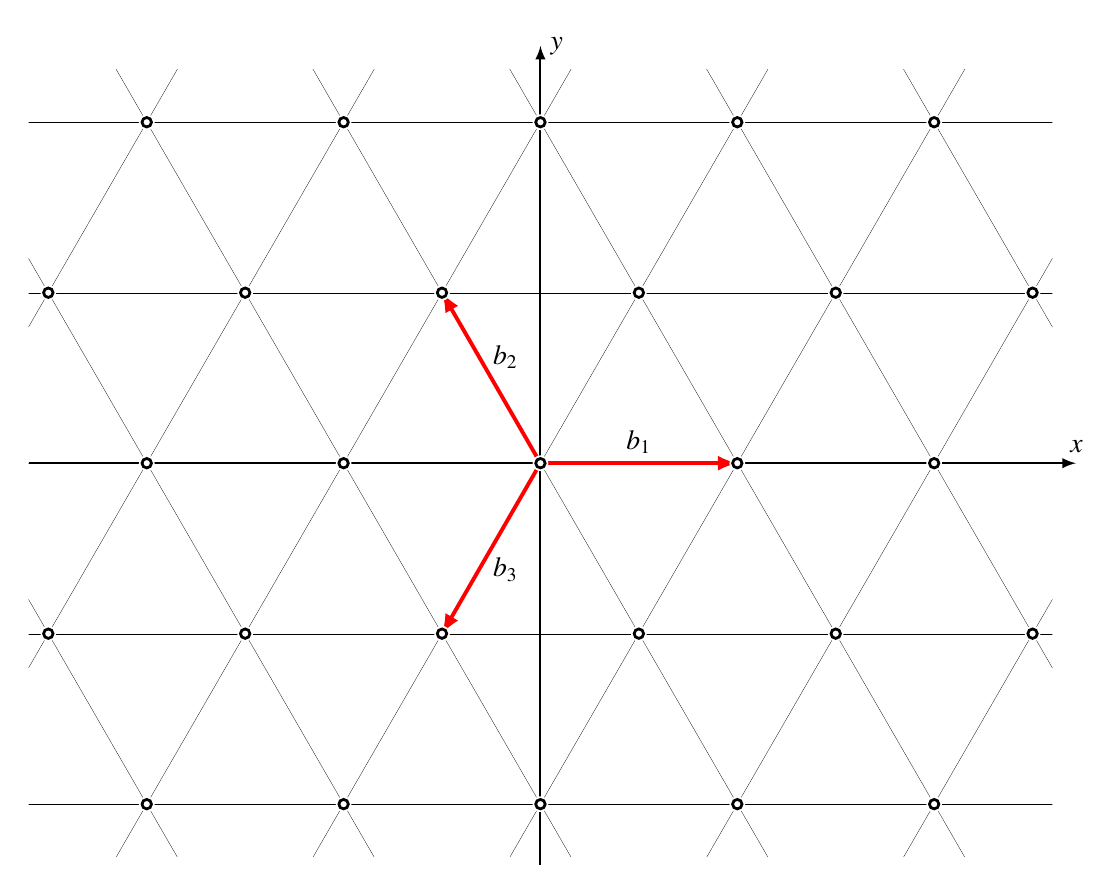
\begin{tikzpicture}[>=latex]

\def\a{2.5}

\def\punkt#1#2{
	\fill[color=white] ({#1},{#2}) circle[radius=0.1];
	\draw[line width=1pt] ({#1},{#2}) circle[radius=0.06];
}

\draw[->,line width=0.7pt] (-6.5,0)--(6.8,0) coordinate[label=$x$];
\draw[->,line width=0.7pt] (0,-5.1)--(0,5.3) coordinate[label={right:$y$}];

\begin{scope}
\clip (-6.5,-5) rectangle (6.5,5);
\foreach \i in{-7,...,7}{
	\draw[line width=0.1pt] (-10,{\i*\a*sqrt(3)/2})--(10,{\i*\a*sqrt(3)/2});
	\draw[line width=0.1pt] ({(\i-5)*\a},{-10*\a*sqrt(3)/2})
		-- ({(\i+5)*\a},{10*\a*sqrt(3)/2});
	\draw[line width=0.1pt] ({(\i-5)*\a},{10*\a*sqrt(3)/2})
		-- ({(\i+5)*\a},{-10*\a*sqrt(3)/2});
}
\end{scope}

\draw[->,line width=1.4pt,color=red] (0,0)--({\a},0);
\draw[->,line width=1.4pt,color=red] (0,0)--({-0.5*\a},{\a*sqrt(3)/2});
\draw[->,line width=1.4pt,color=red] (0,0)--({-0.5*\a},{-\a*sqrt(3)/2});

\node at ({0.5*\a},0) [above] {$b_1$};
\node at ({-0.25*\a-0.1},{\a*sqrt(3)/4}) [above right] {$b_2$};
\node at ({-0.25*\a-0.1},{-\a*sqrt(3)/4}) [below right] {$b_3$};

\begin{scope}
\clip (-6.5,-5) rectangle (6.5,5);
\foreach \x in {-7,...,7}{
	\foreach \y in {-3,...,3}{
		\punkt{\a*(\x+0.5*\y)}{\a*\y*sqrt(3)/2}
	}
}
\end{scope}


\end{tikzpicture}
\end{document}

